%for search with vim and okular
\synctex=1


%%=====================================================================================
% Settings
%%=====================================================================================
\newcommand{\mypapersize}{A4}
\newcommand{\mylaterality}{oneside} %% "oneside" or "twoside"
\newcommand{\myparskip}{half}
\newcommand{\myfontsize}{11pt}
\newcommand{\mylinespread}{singlespacing} % e.g.onehalfspacing, doublespacing, singlespacing
\newcommand{\mylanguage}{french} %american

\documentclass[%
  fontsize=\myfontsize,
	paper=\mypapersize,
	parskip=\myparskip,
	DIV=calc,
	headinclude=true,
	footinclude=true,
	open=right,
	appendixprefix=true,	% include appendix?
	bibliography=totoc,		% include an unnumbered unit of bibliography to the table of contents
	BCOR=10mm,        	  % binding correction (depends on how you bind
	\mylaterality,        % alternative: twoside
  \mylanguage
]{scrbook}

%Encoding
\usepackage[utf8]{inputenc}
\usepackage[T1]{fontenc}

% language adaptions
\usepackage[\mylanguage]{babel}

%% general metadata:
\newcommand{\myauthor}{Valentin Py}  %% also used for PDF metadata (hyperref)
\newcommand{\mydocumentsubject}{Branche }
\newcommand{\mysubject}{Nom du projet}  %% also used for PDF metadata (hyperref)
\newcommand{\myshortsubject}{Nom du projet raccoruci}  %% also used for PDF metadata (hyperref)
\newcommand{\mykeywords}{Consommation, Energie, TLS, Cryptographie}  %% also used for PDF metadata (hyperref)

%% this information is used only for generating the title page:
\newcommand{\myuniversity}{HES-SO Master} %% your university/school
\newcommand{\myfaculty}{HE-Arc} %% your university/school
\newcommand{\myinstitutehead}{Prof 1}
\newcommand{\mysupervisor}{Prof 2}

%%=====================================================================================
% Colors
%%=====================================================================================
% includes some colors
\usepackage[table,usenames,dvipsnames]{xcolor}

% Define some colors used in the template
\definecolor{grey}{gray}{0.95}
\definecolor{dkgreen}{rgb}{0,0.6,0}

\definecolor{mauve}{rgb}{0.58,0,0.82}
\definecolor{red}{rgb}{1,0,0}
\definecolor{DispositionColor}{RGB}{0, 0, 0}



%%=====================================================================================
%% includes pictures --> possible to include them in header/footer
%%=====================================================================================
\usepackage[pdftex]{graphicx}


%%=====================================================================================
%% Style
%%=====================================================================================
% override some list packages that they use babel -> see koma script doc
\usepackage{scrhack}

% nicer quotes
\usepackage[%
  autostyle,          % adapts language setting
  strict,             % turns warnings into errors
  english=american    % use american quotes style
]{csquotes}

\usepackage[automark]{scrpage2}							% allows usage of header and footer
\usepackage[perpage, hang]{footmisc} 				% footnote options

\renewcommand{\headfont}{\normalfont\sffamily\color{DispositionColor}}
\renewcommand{\pnumfont}{\normalfont\sffamily\color{DispositionColor}}
\addtokomafont{disposition}{\color{DispositionColor}}
\addtokomafont{caption}{\color{DispositionColor}\footnotesize}
\addtokomafont{captionlabel}{\color{DispositionColor}}

\usepackage{calc} %% used for calculation of header footer etc. ...

%% change page layout
\addtolength{\oddsidemargin}{-.875in}
\addtolength{\evensidemargin}{-.875in}
\addtolength{\textwidth}{1.75in}
\addtolength{\topmargin}{-.875in}
\addtolength{\textheight}{3in}  %1.75

% header and footer
\pagestyle{scrheadings}							% for customization for header and footer
\renewcommand{\chapterpagestyle}{scrheadings}	% include header and footer on chapter pages
\clearscrheadfoot

% http://ctan.uib.no/macros/latex/contrib/koma-script/doc/scrguien.pdf
% page 204
\ihead{\myshortsubject}
\ifoot{\vspace{-0.25cm}\myauthor}
\ofoot{ \vspace{-0.25cm} \thepage}
\automark{chapter}
\setheadsepline[ \textwidth + 5pt ]{1pt} % seperation line for header...
\setfootsepline[ \textwidth + 5pt ]{1pt} % ... and footer
\setkomafont{footsepline}{\color{red}} 	 % change colors of seperation lines
\setkomafont{headsepline}{\color{red}}

%%=====================================================================================
%% Table on Contents
%%=====================================================================================
\setcounter{tocdepth}{1}
\setcounter{secnumdepth}{1}

\usepackage{makecell}

\usepackage{tabulary}
\newcolumntype{K}[1]{>{\centering\arraybackslash}p{#1}}

\usepackage{verbatim}


%%=====================================================================================
%% bibliography with biber/biblatex
%%=====================================================================================
\usepackage[backend=biber, %% using "biber" to compile references (instead of "biblatex")
            style=numeric, %% see biblatex documentation
            style=alphabetic, %% see biblatex documentation
            backref=true, %% create backlings from references to citations
            natbib=true, %% offering natbib-compatible commands
            hyperref=true,
            sorting=none, %% using hyperref-package references
]{biblatex}

\addbibresource{bib/bibliography.bib}


%%=====================================================================================
%% SIUNITSX -- simplified usage of SI-units
%%=====================================================================================
\usepackage[
            group-digits=false,
            exponent-product = \cdot, % use \cdot instead * for exponent product
            binary-units=true,
            load-configurations=binary,
            load-configurations=abbreviations,
]{siunitx}

% Easy typesetting hex and bin and oct
\usepackage[autolanguage, nosepfour]{numprint}
\usepackage{nbaseprt}

%%=====================================================================================
%% ifthen and todonotes puts to-do-notes in the printed document if you want
%%=====================================================================================
%% used to disable todonotes package
\usepackage{ifthen}
\newboolean{myaddlistoftodos}

\reversemarginpar %To display the todo in the right margin
\setlength{\marginparwidth}{2cm} %To correct the bad placement

\usepackage[english]{todonotes}

%%=====================================================================================
%% Tables, figures, enums, etc...
%%=====================================================================================
%% nice rule's for tables try \toprule \midrule \bottomrule
\usepackage{booktabs}

%% set width of table and more
\usepackage{tabularx}										% creates tables

%% rotate tables and figures
\usepackage{rotating}

%% define caption style
\addtokomafont{caption}{\small} 	% small captions
\usepackage[font=small, width=0.9\textwidth, format=plain, labelfont=bf]{caption}

%%
\usepackage{subfigure}
\usepackage{placeins}

%% customize item look
\usepackage{enumitem}

%%=====================================================================================
%% some utility stuff
%%=====================================================================================
% improved typographical settings
\usepackage[%
    protrusion=true, %
    factor=900       %
]{microtype}

%% switch of extra space after punctuation
\frenchspacing

%% switches to Palatino with small caps and old style figures
\usepackage[%
            sc,%
            osf,%
]{mathpazo}

%% kills space between items
\setlist{noitemsep}

%doc% For additional special characters available by \verb#\ding{}#
\usepackage{pifont}  %% Sonderzeichen fuer Titelseite \ding{}

%doc% This package is required for intelligent spacing after commands
\usepackage{xspace}

%doc% This package offers strikethrough command \verb+\sout{foobar}+.
\usepackage[normalem]{ulem}

%% prevent club & widow penalty
\clubpenalty10000
\widowpenalty10000
\displaywidowpenalty10000




%%=====================================================================================
%% lslistening: used to include source code
%%=====================================================================================
\usepackage{listings}				% include source code

\lstset{% 							% options for representation of source code
  backgroundcolor=\color{grey},   % choose the background color; you must add \usepackage{color} or \usepackage{xcolor}
  basicstyle=\footnotesize,        % the size of the fonts that are used for the code
  breakatwhitespace=false,         % sets if automatic breaks should only happen at whitespace
  breaklines=true,                 % sets automatic line breaking
  captionpos=b,                    % ses the caption-position to bottom
  commentstyle=\color{dkgreen}, % comment style
  deletekeywords={...},            % if you want to delete keywords from the given language
  escapeinside={\%*}{*)},          % if you want to add LaTeX within your code
  frame=lines,                     % adds a frame around the code
  keepspaces=true,                 % keeps spaces in text, useful for keeping indentation of code (possibly needs columns=flexible)
  keywordstyle=\color{blue},       % keyword style
  language=C,                      % the language of the code
  morekeywords={*,...},            % if you want to add more keywords to the set
  numbers=left,                    % where to put the line-numbers; possible values are (none, left, right)
  numbersep=8pt,                   % how far the line-numbers are from the code
  numberstyle=\tiny\color{gray},   % the style that is used for the line-numbers
  rulecolor=\color{black},         % if not set, the frame-color may be changed on line-breaks within not-black text (e.g. comments (green here))
  showspaces=false,                % show spaces everywhere adding particular underscores; it overrides 'showstringspaces'
  showstringspaces=false,          % underline spaces within strings only
  showtabs=false,                  % show tabs within strings adding particular underscores
  stepnumber=1,                    % the step between two line-numbers. If it's 1, each line will be numbered
  stringstyle=\color{blue},        % string literal style
  tabsize=2,                       % sets default tabsize to 2 spaces
  title=\lstname,                  % show the filename of files included with \lstinputlisting; also try caption instead of title
}

%theme for C
\lstdefinestyle{C}{
	language=c, showspaces=false,
	keywordstyle=		\color{blue}\scriptsize,
	commentstyle=	  \color{dkgreen}\scriptsize\sffamily,
	stringstyle=		\color{mauve}\scriptsize,
	title=\lstname,
	escapeinside={//(*}{*)},
	morekeywords={},
	numbers = left, numberstyle=\tiny\color{black}
}

%%=====================================================================================
%% pdfcompresslevel from 0 to 10; std is fine
%%=====================================================================================
\pdfcompresslevel=9

%%=====================================================================================
%% Hyperref should always be the last package added --
%%=====================================================================================
\usepackage[%							% enables typesettings for hyperlinks
	pdftitle={\mysubject},%
	pdfauthor = {\myauthor},%
	pdfsubject = {\mysubject},%
  colorlinks={false},
  pdfcreator={pdfTex},%
  pdfkeywords={\mykeywords},%
  pdftex = true,%
  backref,%
  pagebackref=false, % creates backward references too
  bookmarks=True, %
  bookmarksopen=false, % when starting with AcrobatReader, the Bookmarkcolumn is opened
  pdfpagemode=UseOutlines,% None, UseOutlines, UseThumbs, FullScreen
  plainpages=false % correct, if pdflatex complains: ``destination with same identifier already exists''
]{hyperref}								% should be the last package to be inlcuded!

%---------------------------------------------------------------------------------------------------
% units
%---------------------------------------------------------------------------------------------------
\newcommand{\hexnum}[1]{\texttt{0x#1}}
\newcommand{\code}[1]{\texttt{#1}}

\newcommand{\cm}{\ensuremath{\mathrm{cm}}\xspace}
\newcommand{\m}{\ensuremath{\mathrm{m}}\xspace}
\newcommand{\mm}{\ensuremath{\mathrm{mm}}\xspace}
\newcommand{\microm}{\ensuremath{\mu\mathrm{m}}\xspace}
\newcommand{\s}{\ensuremath{\mathrm{s}}\xspace}
\newcommand{\musec}{\ensuremath{\mu\mathrm{s}}\xspace}


%---------------------------------------------------------------------------------------------------
% include figures
%---------------------------------------------------------------------------------------------------
\newcommand{\myfig}[5]{
\begin{figure}%[htp]
  \begin{center}
     \includegraphics[keepaspectratio,#2]{figures/#1}
     \caption[#4]{#3}
     \label{#5} %% NOTE: always label *after* caption!
  \end{center}
\end{figure}
}



%% ========================================================================
%%  TODO: Enable/Disable
%% ========================================================================
\setboolean{myaddlistoftodos}{false}  %% "true" or "false"
%% If set to "true": the current list of open todos is added after the
%% table of contents. If \mytodonotesoptions is set to "disable", no
%% list of todos is added, independent of this setting here.

%----------------------------------------------------------------------------------------
%	\begin{document}
%----------------------------------------------------------------------------------------
\begin{document}

\frontmatter

% 3 images at the top of the title page
\titlehead{
\begin{minipage}{16cm}
	\centering
	\raisebox{-0.5\height}{
\includegraphics[width=35mm]{../figures/titlepage_fig/hes-so.jpg}}
	\hspace*{1.3cm}
	\raisebox{-0.5\height}{
\includegraphics[width=35mm]{../figures/titlepage_fig/mse.jpg}}
	\hspace*{1.3cm}
	\raisebox{-0.5\height}{
\includegraphics[width=50mm]{../figures/titlepage_fig/he-arc.pdf}}
	\vspace{1.0cm}
\end{minipage}
}

% Add text from #defines.tex
\subject{\mydocumentsubject}
\title{\mysubject}
\author{\myauthor}

\publishers{%\myinstitute\\
						\myfaculty\\
						\myuniversity\\
						\vspace{0.5cm}
						\myinstitutehead\\
						\mysupervisor
}

\maketitle


\cleardoublepage

%----------------------------------------------------------------------------------------
%	Abstract
%----------------------------------------------------------------------------------------
% \include{chapter/00_abstract}
% \clearpage

%----------------------------------------------------------------------------------------
%	List of Contents/Figures/Tables
%----------------------------------------------------------------------------------------
\tableofcontents
%\listoffigures

\ifthenelse{\boolean{myaddlistoftodos}}{
  \newpage\todototoc \listoftodos          %% handy if you are using todonotes with \todo{}
}{}

%----------------------------------------------------------------------------------------
%	Body
%----------------------------------------------------------------------------------------
\mainmatter

% Chapter file here

\chapter{Introduction}

Nihil morati post haec militares avidi saepe turbarum adorti sunt Montium primum, qui divertebat in proximo, levi corpore senem atque morbosum, et hirsutis resticulis cruribus eius innexis divaricaturn sine spiramento ullo ad usque praetorium traxere praefecti.

Ego vero sic intellego, Patres conscripti, nos hoc tempore in provinciis decernendis perpetuae pacis habere oportere rationem. Nam quis hoc non sentit omnia alia esse nobis vacua ab omni periculo atque etiam suspicione belli?

Haec ubi latius fama vulgasset missaeque relationes adsiduae Gallum Caesarem permovissent, quoniam magister equitum longius ea tempestate distinebatur, iussus comes orientis Nebridius contractis undique militaribus copiis ad eximendam periculo civitatem amplam et oportunam studio properabat ingenti, quo cognito abscessere latrones nulla re amplius memorabili gesta, dispersique ut solent avia montium petiere celsorum.


\chapter{Introduction à la Cryptographie}
\section{Principes généraux et termes}
\subsection{Points importants}
\subsubsection{Premier point}


% List
\begin{itemize}
	\item fonction de hachage,
	\item cryptographie symétrique,
	\item cryptographie asymétrique,
	\item infrastructures à clé publique (certificats).
\end{itemize}

% Figure with caption and label
\begin{figure}[h]
\centering
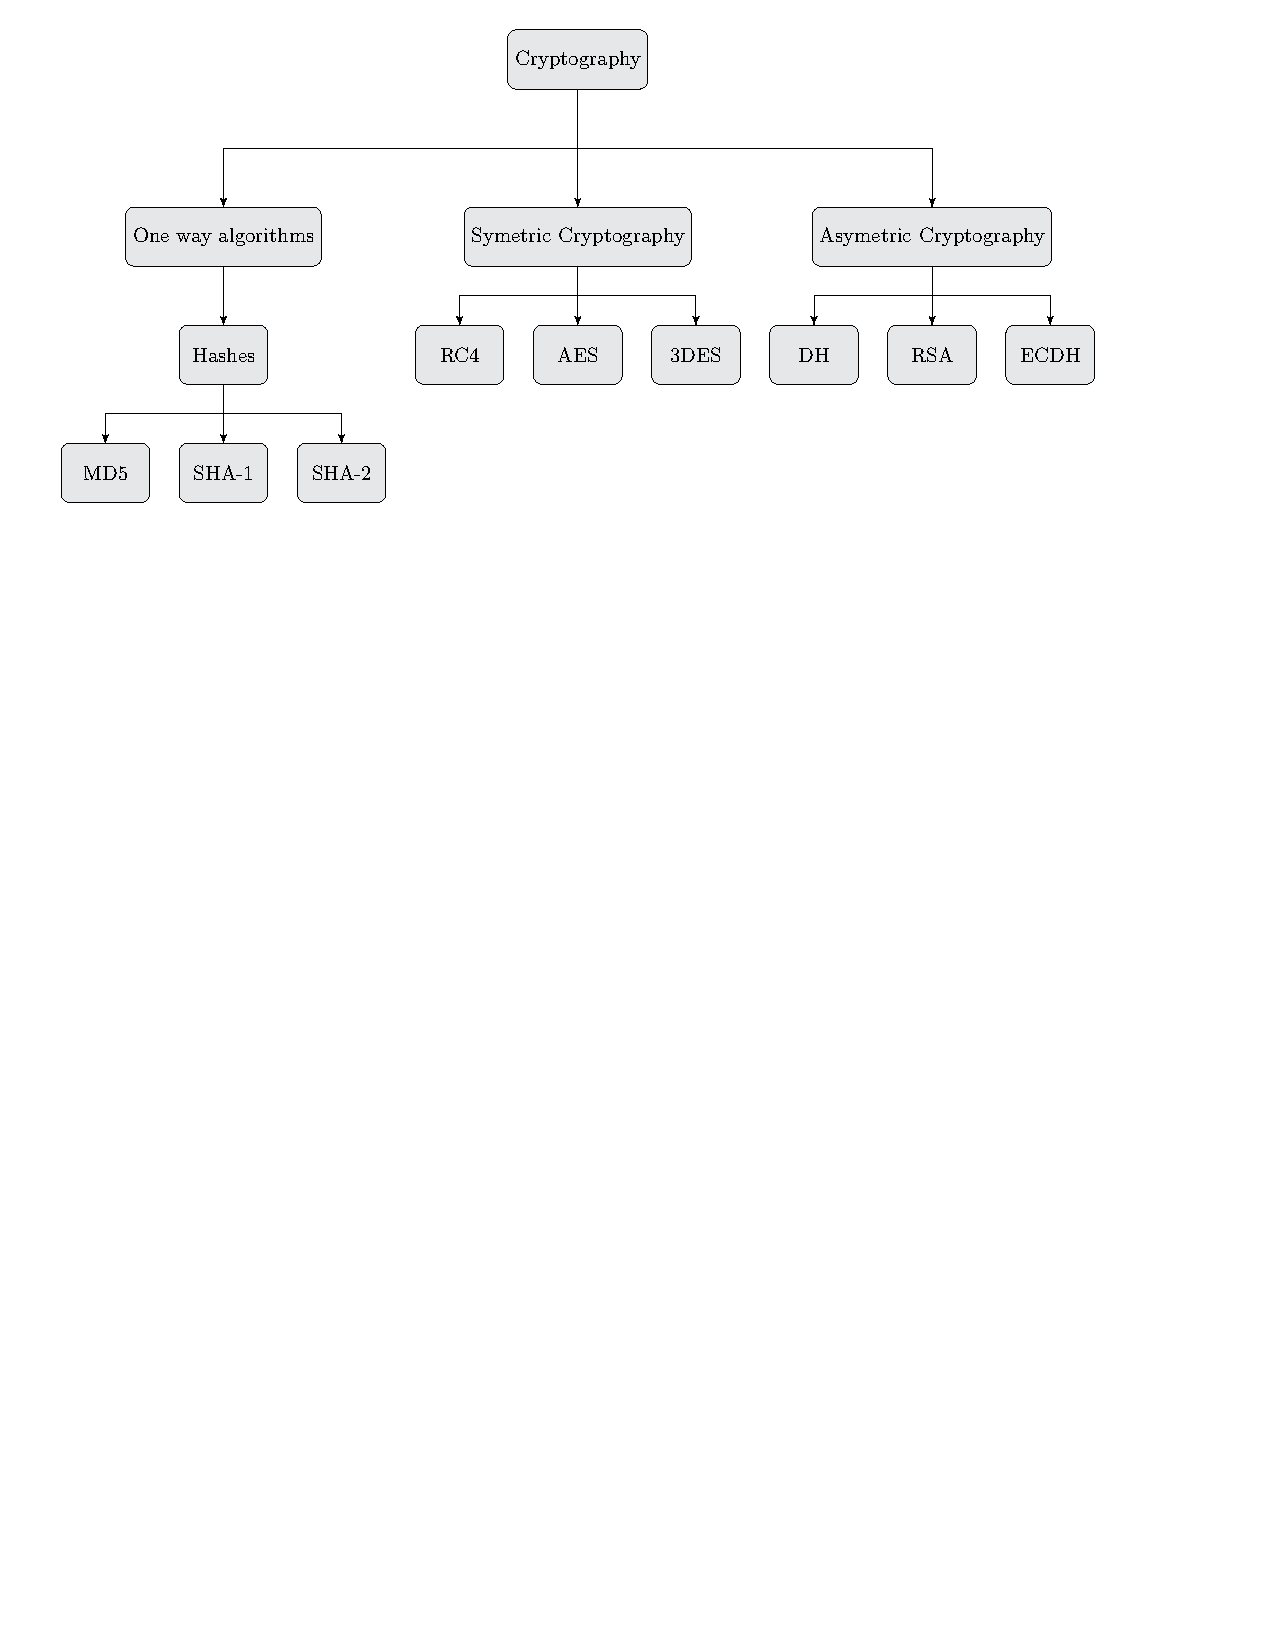
\includegraphics[trim= 0cm 19cm 3cm 0, clip,width=0.8\textwidth]{../figures/flowcharts/crypto_types.pdf}
\caption[Algorithmes de cryptographie importants]{Algorithmes de cryptographie importants}
\label{fig:crypto_algos}
\end{figure}
\FloatBarrier

% Table
\begin{table}[h]
	\vspace{0.5cm}
	% 3 columns + width of each column
		\begin{tabular}{|p{3cm}|p{4cm}|p{9cm}|}
		\hline
		%First line + bold horizontal line
		Nom & Taille du hash & Remarque \\ \Xhline{5\arrayrulewidth}
		MD5 & 128 bits  &  Déprécié \\ \hline
		SHA-1 & 160 bits & Déprécié par certains organismes (BSI\footnotemark[1], etc)  \\ \hline
		SHA-2 & 256 / 384 / 512 bits, dépend de la version utilisée & Recommandé \\ \hline
		\end{tabular}
	\caption{Caractéristiques des trois familles de fonctions de hachage}
	\label{hash_caracteristics}
\end{table}


% Quote from bibliography
% Reference to figure
Tous ces concepts sont expliqués en détail dans le livre \cite{understanding_cryp} ou à la figure \ref{fig:crypto_algos}.

%New page
\clearpage
% \cleardoublepage

% To prevent figures to be placed too far away
% Often used just after a figure or at the end of a section / subsection ,...
\FloatBarrier

% Footnote
\footnotetext[1]{Bundesamt für Sicherheit in der Informationstechnik, Allemagne}

% Todo
\todo[inline]{TODO: Remove this illustration}

%Source code inclusion
\lstinputlisting[linerange={104-128}, caption={sample C code - sample.c}, label={lst:sample}]{../source_code/sample.c}

\include{chapter/20_TLS}

\chapter{Conclusion}
Nihil morati post haec militares avidi saepe turbarum adorti sunt Montium primum, qui divertebat in proximo, levi corpore senem atque morbosum, et hirsutis resticulis cruribus eius innexis divaricaturn sine spiramento ullo ad usque praetorium traxere praefecti.

Ego vero sic intellego, Patres conscripti, nos hoc tempore in provinciis decernendis perpetuae pacis habere oportere rationem. Nam quis hoc non sentit omnia alia esse nobis vacua ab omni periculo atque etiam suspicione belli?

Haec ubi latius fama vulgasset missaeque relationes adsiduae Gallum Caesarem permovissent, quoniam magister equitum longius ea tempestate distinebatur, iussus comes orientis Nebridius contractis undique militaribus copiis ad eximendam periculo civitatem amplam et oportunam studio properabat ingenti, quo cognito abscessere latrones nulla re amplius memorabili gesta, dispersique ut solent avia montium petiere celsorum.


%----------------------------------------------------------------------------------------
%	Bibliography
%----------------------------------------------------------------------------------------

%% prints every entry of the bib file -- useful in a state where is no cite
\appendix
\nocite{*}
\printbibliography


%----------------------------------------------------------------------------------------
%	\end{document}
%----------------------------------------------------------------------------------------
\end{document}
